\subsection{Invertible Bimodules and Morita Equivalence}

DEFINITION 1. --- Let A and B be k-algebras and P an \((\mathrm{A},\mathrm{B})_{k}\) -bimodule. We say that P is invertible if there exists a \((\mathrm{B},\mathrm{A})_{k}\) -bimodule Q such that \(P \otimes_{B} Q\) is isomorphic to \(_{s}A_{d}\) and \(Q \otimes_{A} P\) to \(_{s}B_{d}\) . Such a bimodule Q is called an inverse of P.

Let A and B be k-algebras, and let P be an invertible \((\mathrm{A},\mathrm{B})_{k}\) -bimodule. Let C be a k-algebra and \(P'\) an invertible \((\mathrm{B},\mathrm{C})_{k}\) -bimodule. Finally, let Q and \(Q'\) be inverse bimodules of P and \(P'\) , respectively. By the associativity of the tensor product (II, §3, No.~8, p.~258, Proposition 8) and Proposition 4 of II, §3, No.~4, p.~249, the \((\mathrm{C},\mathrm{A})_{k}\) -bimodule \(Q'\otimes_{B}Q\) is an inverse of the \((\mathrm{A},\mathrm{C})_{k}\) -bimodule \(P\otimes_{B}P'\) , so that \(P\otimes_{B}P'\) is an invertible \((\mathrm{A},\mathrm{C})_{k}\) -bimodule. Hence, the relation

``A and B are k-algebras, and there exists an invertible \((A,B)_{k}\) -bimodule'' is an equivalence relation.

DEFINITION 2. --- Two k-algebras A and B are called Morita equivalent if there exists an invertible \((\mathrm{A},\mathrm{B})_{k}\) -bimodule. Rings A and B are called Morita equivalent if the Z-algebras A and B are Morita equivalent.

Two isomorphic k-algebras are Morita equivalent. If two k-algebras are Morita equivalent, then their opposite algebras are Morita equivalent.

Let P be an invertible \((\mathrm{A},\mathrm{B})_{k}\) -bimodule and Q an inverse of P. Then Q is an invertible \((\mathrm{B},\mathrm{A})_{k}\) -bimodule, and it has P as inverse. Moreover, viewed as a \((\mathrm{B}^{\circ},\mathrm{A}^{\circ})_{k}\) -bimodule, P is invertible and has the \((\mathrm{A}^{\circ},\mathrm{B}^{\circ})_{k}\) -bimodule Q as inverse.

Lemma 1. --- Let A and B be k-algebras, P be an invertible \((\mathrm{A},\mathrm{B})_{k}\) -bimodule, M and N be B-modules, and \(u:M\to N\) be a B-linear mapping. If the mapping \(1_{P}\otimes u:P\otimes_{B}M\to P\otimes_{B}N\) is zero (resp. bijective), then so is u.

Let Q be a bimodule inverse to P and \(\theta: Q \otimes_{A} P \to_{s} B_{d}\) an isomorphism of \((B, B)_{k}\) -bimodules. The lemma follows from the commutativity of the diagram

\pandocbounded{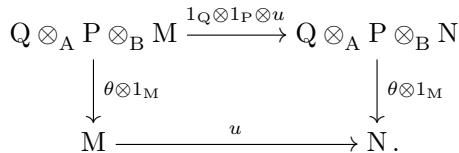
\includegraphics[keepaspectratio]{images/part001_2598f5b2.jpg}}

THEOREM 1. --- Let A and B be k-algebras and P an \((A,B)_{k}\) -bimodule. Denote the \((B,A)_{k}\) -bimodule \(\operatorname{Hom}_{\mathrm{A}}(\mathrm{P},\mathrm{A}_{s})\) by \(P^{*}\) . The following properties are equivalent:

\begin{enumerate}
\def\labelenumi{(\roman{enumi})}
\item
  The \((\mathrm{A},\mathrm{B})_k\) -bimodule P is invertible.
\item
  The A-module P is projective, finitely generated, and generating, and the mapping \(b \mapsto b_{P}\) from B to \(\operatorname{End}_{\mathrm{A}}(\mathrm{P})^{\circ}\) is a k-algebra isomorphism.
\item
  The right B-module P is projective, finitely generated, and generating, and the mapping \(a \mapsto a_{P}\) from A to \(\operatorname{End}_{\mathrm{B}}(\mathrm{P})\) is a k-algebra isomorphism. If these properties hold, then the homomorphisms
\end{enumerate}

\[
\Theta : \mathrm{P} ^ {*} \otimes \mathrm{P} \to {} _ {s} \mathrm{B} _ {d} \quad \text{and} \quad \Lambda : \mathrm{P} \otimes \mathrm{P} ^ {*} \to {} _ {s} \mathrm{A} _ {d}
\]

are isomorphisms, so that the \((\mathrm{B},\mathrm{A})_k\) -bimodule \(\mathrm{P}^*\) is an inverse of \(\mathrm{P}\) .

If property (ii) holds, then P is an invertible \((\mathrm{A},\mathrm{B})_{k}\) -bimodule with inverse \(P^{*}\) (VIII, p.~98, Proposition 2 and p.~98, Proposition 3). This proves that (ii) implies (i) and the last assertion.

Suppose that the \((\mathrm{A},\mathrm{B})_{k}\) -bimodule P is invertible. Then the A-module P is generating (VIII, p.~98, Proposition 3, (iii) \(\Rightarrow\) (i)). It is therefore faithful and balanced (VIII, p.~82, Theorem 2) and, consequently, the mapping \(a \mapsto a_{p}\) from A to \(\operatorname{End}_{\mathrm{B}}(\mathrm{P})\) is bijective.

Let us now prove that the mapping \(b \mapsto b_{\mathrm{P}}\) from B to \(\mathrm{End}_{\mathrm{A}}(\mathrm{P})\) is bijective. Let Q be a \((\mathrm{B},\mathrm{A})_k\) -bimodule, inverse to P. Let \(u \in \mathrm{End}_{\mathrm{A}}(\mathrm{P})\) ; then \(1_{\mathrm{Q}} \otimes u\) is an endomorphism of the left B-module \(\mathbf{Q} \otimes_{\mathrm{A}} \mathbf{P}\) . Since the \((\mathrm{B},\mathrm{B})_k\) -bimodule \(\mathbf{Q} \otimes_{\mathrm{A}} \mathbf{P}\) is isomorphic to \({}_s\mathbf{B}_d\) , there exists a unique element \(b\) of B such that \(1_{\mathrm{Q}} \otimes u\) is the homothety with ratio \(b\) of the right B-module \(\mathbf{Q} \otimes_{\mathrm{A}} \mathbf{P}\) . Consequently, we have \(1_{\mathrm{Q}} \otimes (u - b_{\mathrm{P}}) = 0\) . Hence, \(u = b_{\mathrm{P}}\) by Lemma 1; this proves that the mapping \(b \mapsto b_{\mathrm{P}}\) from B to \(\operatorname{End}_{\mathrm{A}}(\mathrm{P})\) is bijective.

By Proposition 2 of VIII, p.~98, the A-module P is then projective and finitely generated. We have therefore proved the equivalence of (i) and (ii).

By interchanging the roles of A and B, we obtain the equivalence of (i) and (iii), which concludes the proof of the proposition.

COROLLARY 1. --- Let A and B be Morita equivalent k-algebras, and let P be an invertible \((A,B)_{k}\) -bimodule. There exists an isomorphism \(\varphi\) from the center \(Z(A)\) of A to the center of B determined by the relation \(\varphi(z)_{\mathrm{P}} = z_{\mathrm{P}}\) for every \(z \in Z(A)\) . The automorphisms of the \((A,B)_{k}\) -bimodule P are the homotheties \(z_{P}\) where z is an invertible element of \(Z(A)\) .

Given Theorem 1, this follows from Remark 2 of VIII, p.~97.

COROLLARY 2. --- Let A and B be Morita equivalent k-algebras, and let P be an invertible \((\mathrm{A},\mathrm{B})_{k}\) -bimodule. Every \((\mathrm{B},\mathrm{A})_{k}\) -bimodule inverse to P is isomorphic to the dual \(\mathrm{P}^{*}=\mathrm{Hom}_{\mathrm{A}}(\mathrm{P},\mathrm{A})\) of P. More precisely, let Q be a \((\mathrm{B},\mathrm{A})_{k}\) -bimodule that is an inverse of P, and let \(\lambda:P\otimes_{B}Q\to_{s}A_{d}\) be an isomorphism of \((\mathrm{A},\mathrm{A})_{k}\) -bimodules. There exists a unique mapping \(\tau:\mathrm{Q}\to\mathrm{P}^{*}\) determined by the relation \(\langle p,\tau(q)\rangle=\lambda(p\otimes q)\) for \(p\in P\) and \(q\in Q\) , and \(\tau\) is an isomorphism of \((\mathrm{B},\mathrm{A})_{k}\) -bimodules.

The existence and uniqueness of the mapping \(\tau\) are clear. It is a homomorphism of \((\mathrm{B},\mathrm{A})_{k}\) -bimodules, and we have \(\lambda=\Lambda\circ(1_{\mathrm{P}}\otimes\tau)\) . Since \(\lambda\) and \(\Lambda\) are isomorphisms of \((\mathrm{A},\mathrm{A})_{k}\) -bimodules (VIII, p.~101, Theorem 1), so is \(1_{P}\otimes\tau\) . By Lemma 1, the mapping \(\tau\) is bijective.

Remark. --- Under the assumptions of the corollary, let q be an element of Q such that we have \(\lambda(p \otimes q) = 0\) for every \(p \in P\) . We then have \(\tau(q) = 0\) , that is, q = 0. Likewise, if p is an element of P such that we have \(\lambda(p \otimes q) = 0\) for every \(q \in Q\) , then p = 0.

Examples. --- 1) Let B be a \(k\) -algebra, \(n\) an integer \(\geqslant 1\) , and A the \(k\) -algebra \(\mathbf{M}_n(\mathrm{B})\) . The right B-module \(\mathrm{P} = \mathrm{B}_d^n\) is projective, finitely generated, and generating, and A can be identified with the endomorphism algebra of P (II, §10, No.~7, p.~349). By Theorem 1, the \((\mathrm{A},\mathrm{B})_k\) -bimodule P is invertible. The algebras B and \(\mathbf{M}_n(\mathrm{B})\) are therefore Morita equivalent.

\begin{enumerate}
\def\labelenumi{\arabic{enumi})}
\setcounter{enumi}{1}
\tightlist
\item
  *Let A be a commutative \(k\) -algebra and P an A-module. We view P as an \((A, A)_k\) -bimodule whose two laws of action are equal. If the \((A, A)_k\) -bimodule P is invertible, then the A-module P is finitely generated (Theorem 1). By Theorem 3 of Comm. Alg., II, §5, No.~4, p.~114, the following properties are equivalent:
\end{enumerate}

\begin{enumerate}
\def\labelenumi{(\roman{enumi})}
\item
  The \((\mathrm{A},\mathrm{A})_{k}\) -bimodule P is invertible.
\item
  There exists an A-module \(\mathrm{Q}\) such that \(\mathrm{P} \otimes_{\mathrm{A}} \mathrm{Q}\) is isomorphic to \(\mathrm{A}\) .
\item
  The A-module P is projective, finitely generated, and of rank 1. *
\end{enumerate}

